\chapter{Urlaub und Abwesenheit}
\label{cha:holidays}

Die Abwesenheiten von Helfenden kann auf zwei Arten im Portal hinterlegt werden:
\begin{enumerate}
	\item Urlaub oder Abwesenheit über einen Zeitraum. Hierfür muss über das Menü  die Seite \glqq Abwesenheit\grqq{} aufgerufen werden welche die Möglichkeit bietet alle aktuellen und zukünftigen Abwesenheiten zu bearbeiten oder neue anzulegen.
	
	\begin{figure}[h]
		\begin{addmargin}{-0.2\linewidth}
			\centering 
			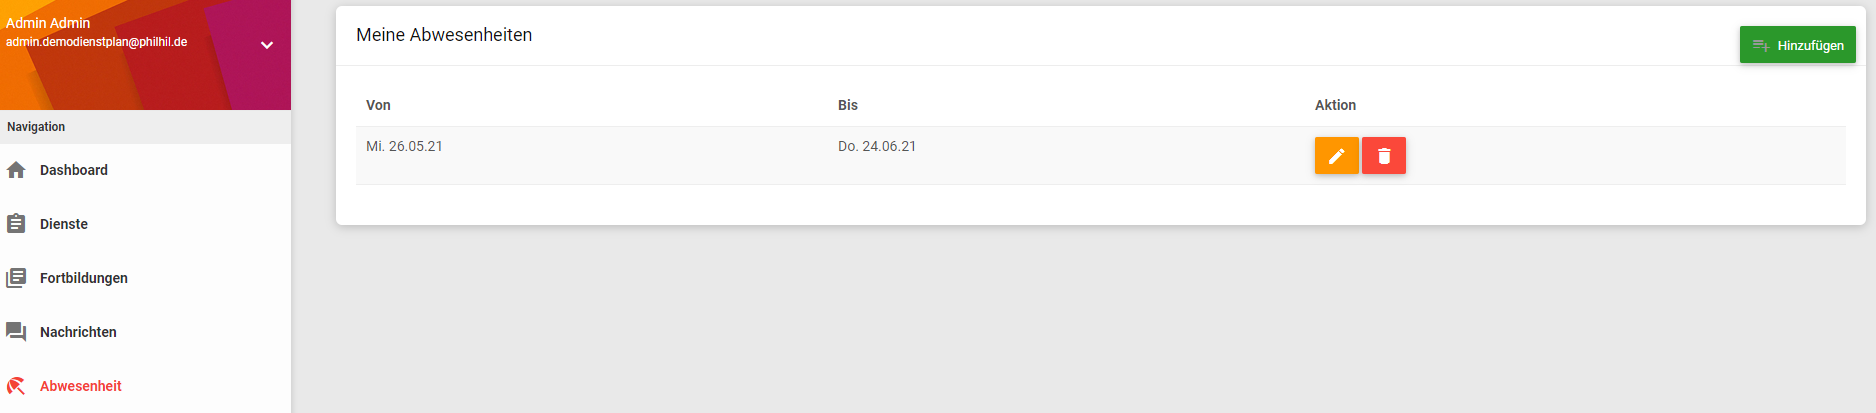
\includegraphics[width=15cm]{Bilder/view_holidays.png}
		\end{addmargin} 
		\caption[Urlaub und Abwesenheit]{Übersicht Abwesenheiten}
		\label{fig:view_holidays}
	\end{figure}
	
	\item Abwesenheit oder nicht Verfügbarkeit für einen einzelnen Dienst bzw. Tag. Für jeden Dienst oder Fortbildung kann rechts oben über die drei kleinen Punkte \glqq Keine Zeit\grqq{} gewählt werden. Dies erstellt automatisch einen Eintrag in den Abwesenheiten mit dem Datum des jeweiligen Dienstes.
	
	\begin{figure}[h]
		\begin{addmargin}{-0.2\linewidth}
			\centering 
			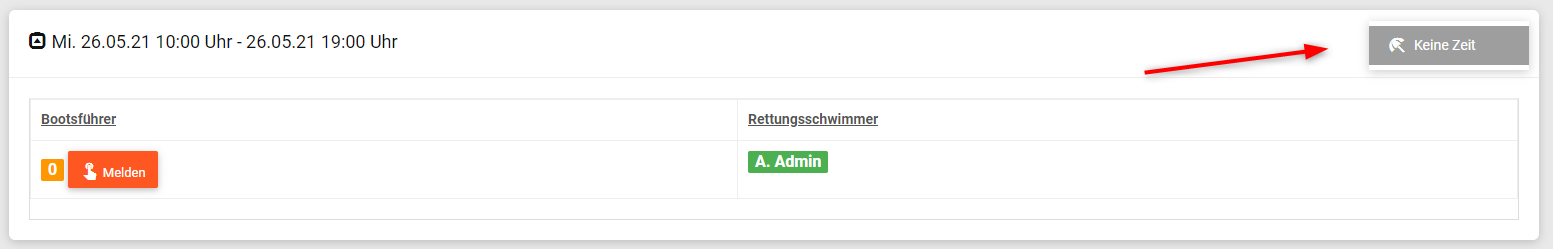
\includegraphics[width=15cm]{Bilder/view_service_holiday.png}
		\end{addmargin} 
		\caption[Abwesenheit]{Nicht verfügbar für einen Dienst / Tag}
		\label{fig:view_service_holiday}
	\end{figure}
\end{enumerate}


Alle Dienste und Fortbildungen, welche in einem Abwesenheits-Zeitraum liegen, werden in der jeweiligen Übersicht grau dargestellt. Die Dienstplan-Verwalter sehen ebenfalls, ob ein User im Urlaub ist. Der User kann sich trotzdem jederzeit für einen Dienst melden. 